\section{Abstrahierung}

Im nachfolgenden Teil wird die Umsetzung der folgenden Use Cases beschrieben. Die Use Cases sind nach der Nummerierung priorisiert worden. Der UC01 soll auf jeden Fall umgesetzt werden. Der UC02 muss evaluiert werden, ob dies mit der API des DNA Centers im Zusammenspiel mit dem ENCS überhaupt möglich ist. Zum Schluss kommt der UC03, welcher nur optional ist und bei genügend verbleibender Zeit implementiert wird.

\subsection{Use Cases Brief}

\subsubsection{UC01: Network Orchestration}
Ein Administrator kann in einem Web Interface Netzwerke erstellen und verwalten. Des Weiteren ist die Möglichkeit gegeben, Policies, welche die Kommunikation zwischen diesen Netzen regeln zu erstellen. Die entsprechenden Konfigurationen werden auf allen beteiligten Geräten automatisch via APIs erstellt.

\subsubsection{UC02: ENCS Virtual Machine Management}
Ein Administrator kann in einem Web Interface die VMs auf einem ENCS System verwalten.

\subsubsection{UC03: Configuration History}
Ein Web Interface bietet die Möglichkeit, die Konfigurationen aller Geräte innerhalb einer Fabric anzuzeigen. Des weiteren kann die aktuelle Konfiguration mit älteren Versionen der Konfiguration verglichen werden.

\subsection{Use Cases Fully Dressed}

\subsubsection{UC01: Network Orchestration}
\begin{table}[H]
	\rowcolors{2}{gray!25}{white}
	\centering
	\begin{tabularx}{\textwidth}{l | X}
		Primary Actor      & Administrator        \\
		\hline
		Beschreibung       & Ein Administrator kann in einem Web Interface Netzwerke erstellen und verwalten. Des Weiteren ist die Möglichkeit gegeben, Policies, welche die Kommunikation zwischen diesen Netzen regeln zu erstellen. Die entsprechenden Konfigurationen werden auf allen beteiligten Geräten automatisch via APIs erstellt. \\ 
		\hline
		Stakeholders       &  
		\begin{itemize}	
			\item Administrator
			\item User
		\end{itemize}              \\
		\hline
		Preconditions      & 
		\begin{itemize}	
			\item DNA Center komplett konfiguriert
			\item Die Fabric läuft ohne Einschränkung
			\item Web Interface steht zur Verfügung
		\end{itemize}  \\
		\hline
		Postconditions     & 
		\begin{itemize}	
			\item Änderungen an Netzen wurden auf den Netzwerkdevices umgesetzt
			\item Policies sind korrekt umgesetzt
		\end{itemize}  \\
		\hline
		Main Success Story & 
		\begin{enumerate}
			\item Ein Netzwerk wird erstellt
			\item Die Software erstellt das Netzwerk auf allen nötigen Netzwerkgeräten
			\item Eine Policy für die Kommunikation mit anderen Netzen wird definiert
			\item Die Konfiguration für die Policy wird automatisch auf allen nötigen Netzwerkgeräten erstellt
		\end{enumerate}
		\\
		\hline
		Alternative Flows  & 
		\begin{itemize}
			\item[1a.] Ein Netzwerk wird gelöscht
			\item[1b.] Eine Policy wird verändert
		\end{itemize}
	\end{tabularx}
	\caption{UC01 Fully Dressed}
	\label{tab:UC01}
\end{table}

\subsubsection{UC02: ENCS Virtual Machine Management}
\begin{table}[H]
	\rowcolors{2}{gray!25}{white}
	\centering
	\begin{tabularx}{\textwidth}{l | X}
		Primary Actor      & Administrator        \\
		\hline
		Beschreibung       & Ein Administrator kann in einem Web Interface die VMs auf einem ENCS System verwalten. \\ 
		\hline
		Stakeholders       &  
		\begin{itemize}	
			\item Administrator
		\end{itemize}              \\
		\hline
		Preconditions      & 
		\begin{itemize}	
			\item ENCS ist konfiguriert und mit dem DNA Center verbunden
			\item VM Profile existieren
		\end{itemize}  \\
		\hline
		Postconditions     & 
		\begin{itemize}	
			\item VMs befinden sich im gewünschten Zustand
		\end{itemize}  \\
		\hline
		Main Success Story & 
		\begin{enumerate}
			\item Eine VM wird erstellt
			\item Eine VM wird gestartet
			\item VM wird einem Netzwerk zugewiesen
		\end{enumerate}
		\\
		\hline
		Alternative Flows  & 
		\begin{itemize}
			\item[1a.] VM wird gelöscht
		\end{itemize}
	\end{tabularx}
	\caption{UC02 Fully Dressed}
	\label{tab:UC02}
\end{table}

\subsubsection{UC03: Configuration History}
\begin{table}[H]
	\rowcolors{2}{gray!25}{white}
	\centering
	\begin{tabularx}{\textwidth}{l | X}
		Primary Actor      & Administrator        \\
		\hline
		Beschreibung       & Ein Web Interface bietet die Möglichkeit, die Konfigurationen aller Geräte innerhalb einer Fabric anzuzeigen. Des weiteren kann die aktuelle Konfiguration mit älteren Versionen der Konfiguration verglichen werden. \\ 
		\hline
		Stakeholders       &  
		\begin{itemize}	
			\item Administrator
		\end{itemize}              \\
		\hline
		Preconditions      & 
		\begin{itemize}	
			\item Netzwerkgeräte sind erreichbar
		\end{itemize}  \\
		\hline
		Postconditions     & 
		\begin{itemize}	
			\item Konfiguration wird angezeigt
		\end{itemize}  \\
		\hline
		Main Success Story & 
		\begin{enumerate}
			\item Ein Netzwerkgerät wird gewählt
			\item Ein Zeitpunkt wird gewählt
			\item Konfiguration zum gewählten Zeitpunkt kann mit der aktuellen Version verglichen werden
		\end{enumerate}
		\\
		\hline
		Alternative Flows  & 
	\end{tabularx}
	\caption{UC03 Fully Dressed}
	\label{tab:UC03}
\end{table}

\subsection{Technologien}
Für das entwickeln des Orchestrierungstool wird Python verwendet. Für das Web Interface wird das Framework Flask eingesetzt. Mit diesen Technologien wird eine Web Anwendung entwickelt, die mit Hilfe der APIs des DNA Centers, des ENCS und der Netzwerkgeräte einzelne Prozesse vereinfacht oder automatisiert.

\subsubsection{Python}
Python ist eine objektorientierte Programmiersprache. Die einfache und leicht erlernbare Python-Syntax hebt die Lesbarkeit hervor und reduziert dadurch die Programmwartung. Python unterstützt Module und Pakete, was die Modularität von Programmen und die Wiederverwendung von Code fördert. Der Python-Interpreter und die umfangreiche Standardbibliothek sind in Quell- oder Binärform kostenlos für alle gängigen Plattformen verfügbar und können frei verteilt werden. \cite{python}

\subsubsection{Flask}
Flask ist ein in Python geschriebenes Webframework. Der Fokus von Flask liegt auf Erweiterbarkeit und guter Dokumentation. Die einzigen Abhängigkeiten sind Jinja2, eine Template-Engine und Werkzeug, eine Bibliothek zum Erstellen von WSGI-Anwendungen. \cite{flask}

\subsubsection{DNA Center Platform}
Cisco hat seit dem Sommer 2018 die DNA Center Platform zur Verfügung gestellt, über die nun auf den API Katalog und andere Ressourcen zugegriffen werden kann. So können beispielsweise die Platform Funktionen auch verwendet werden, um die Bereitstellung und Verwaltung von Netzwerken zu vereinfachen.


So soll das DNA Center nun eine 360 Grad Erweiterbarkeit durch vier verschiedene Platform Funktionen bereitstellen. Dazu gehören die Intent-based APIs, Process adapters, Domain adapters, sowie SDKs. \cite{dnac-platform}

\begin{figure}[H]
	\centering
	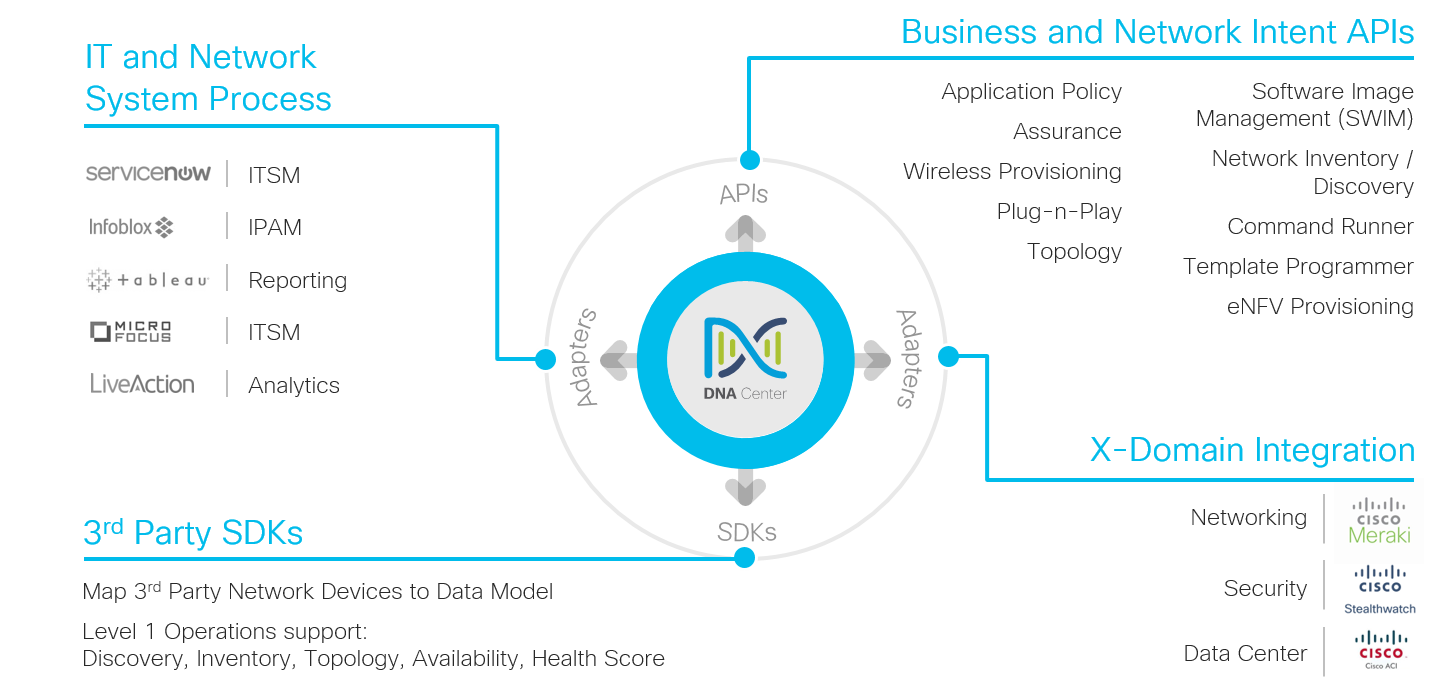
\includegraphics[width=0.8\linewidth]{img/Abstrahierung/dnac-platform}
	\caption{DNA Center Plattform \cite{dnac-platform}}
	\label{fig:DNA Center Plattform}
\end{figure}


\paragraph{Intent-API}

Die Intent-API ist eine Northbound REST API, welche bestimmte Funktionen des DNA Centers verfügbar macht. Mit der RESTful Intent API des DNA Centers können die HTTP- (GET, POST, PUT, DELETE) und JSON-Syntax verwendet werden, um das Netzwerk zu analysieren und zu konfigurieren. \cite{dnac-platform}

Diese APIs findet man im DNA Center unter \textit{Platform $\rightarrow$ Developer Toolkit $\rightarrow$ APIs}

\begin{figure}[H]
	\centering
	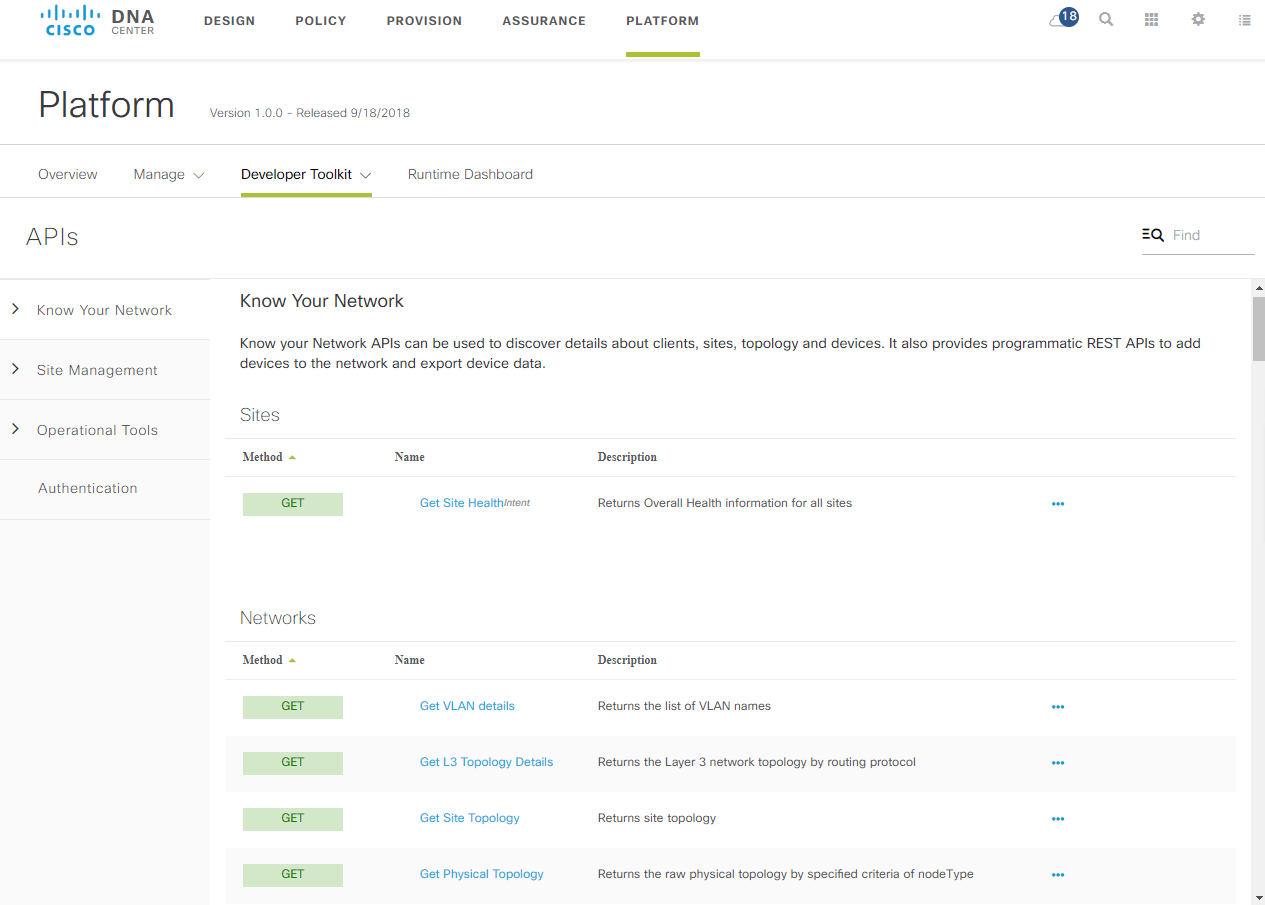
\includegraphics[width=0.8\linewidth]{img/Abstrahierung/dnac-apis}
	\caption{DNA Center Plattform APIs}
	\label{fig:DNA Center Plattform APIs}
\end{figure}

\subsubsection{ENCS/NFVIS API}
Der ENCS beziehungsweise die NFVIS, welche auf dem ENCS läuft, stellt ebenfalls eine programmierbare API für Service Orchestration mittels REST- und NETCONF-API bereit. 

Die API Dokumentationen sind bei NFVIS leider nicht direkt über dessen Applikation verfügbar. Es gibt jedoch eine Dokumentation von Cisco direkt, welche unter dem Namen \textit{API Reference for Cisco Enterprise Network Function Virtualization Infrastructure Software} \cite{nfvis-api} zu finden ist.


\subsection{Umsetzung}

\subsubsection{Ablauf Erstellung Netzwerk}
Um die Erstellung eines Netzwerkes zu vereinfachen, wird ein Wizard erstellt, mit welchem folgende einzelnen Schritte vereinfacht auszuführen sind. 

\begin{figure}[H]
	\centering
	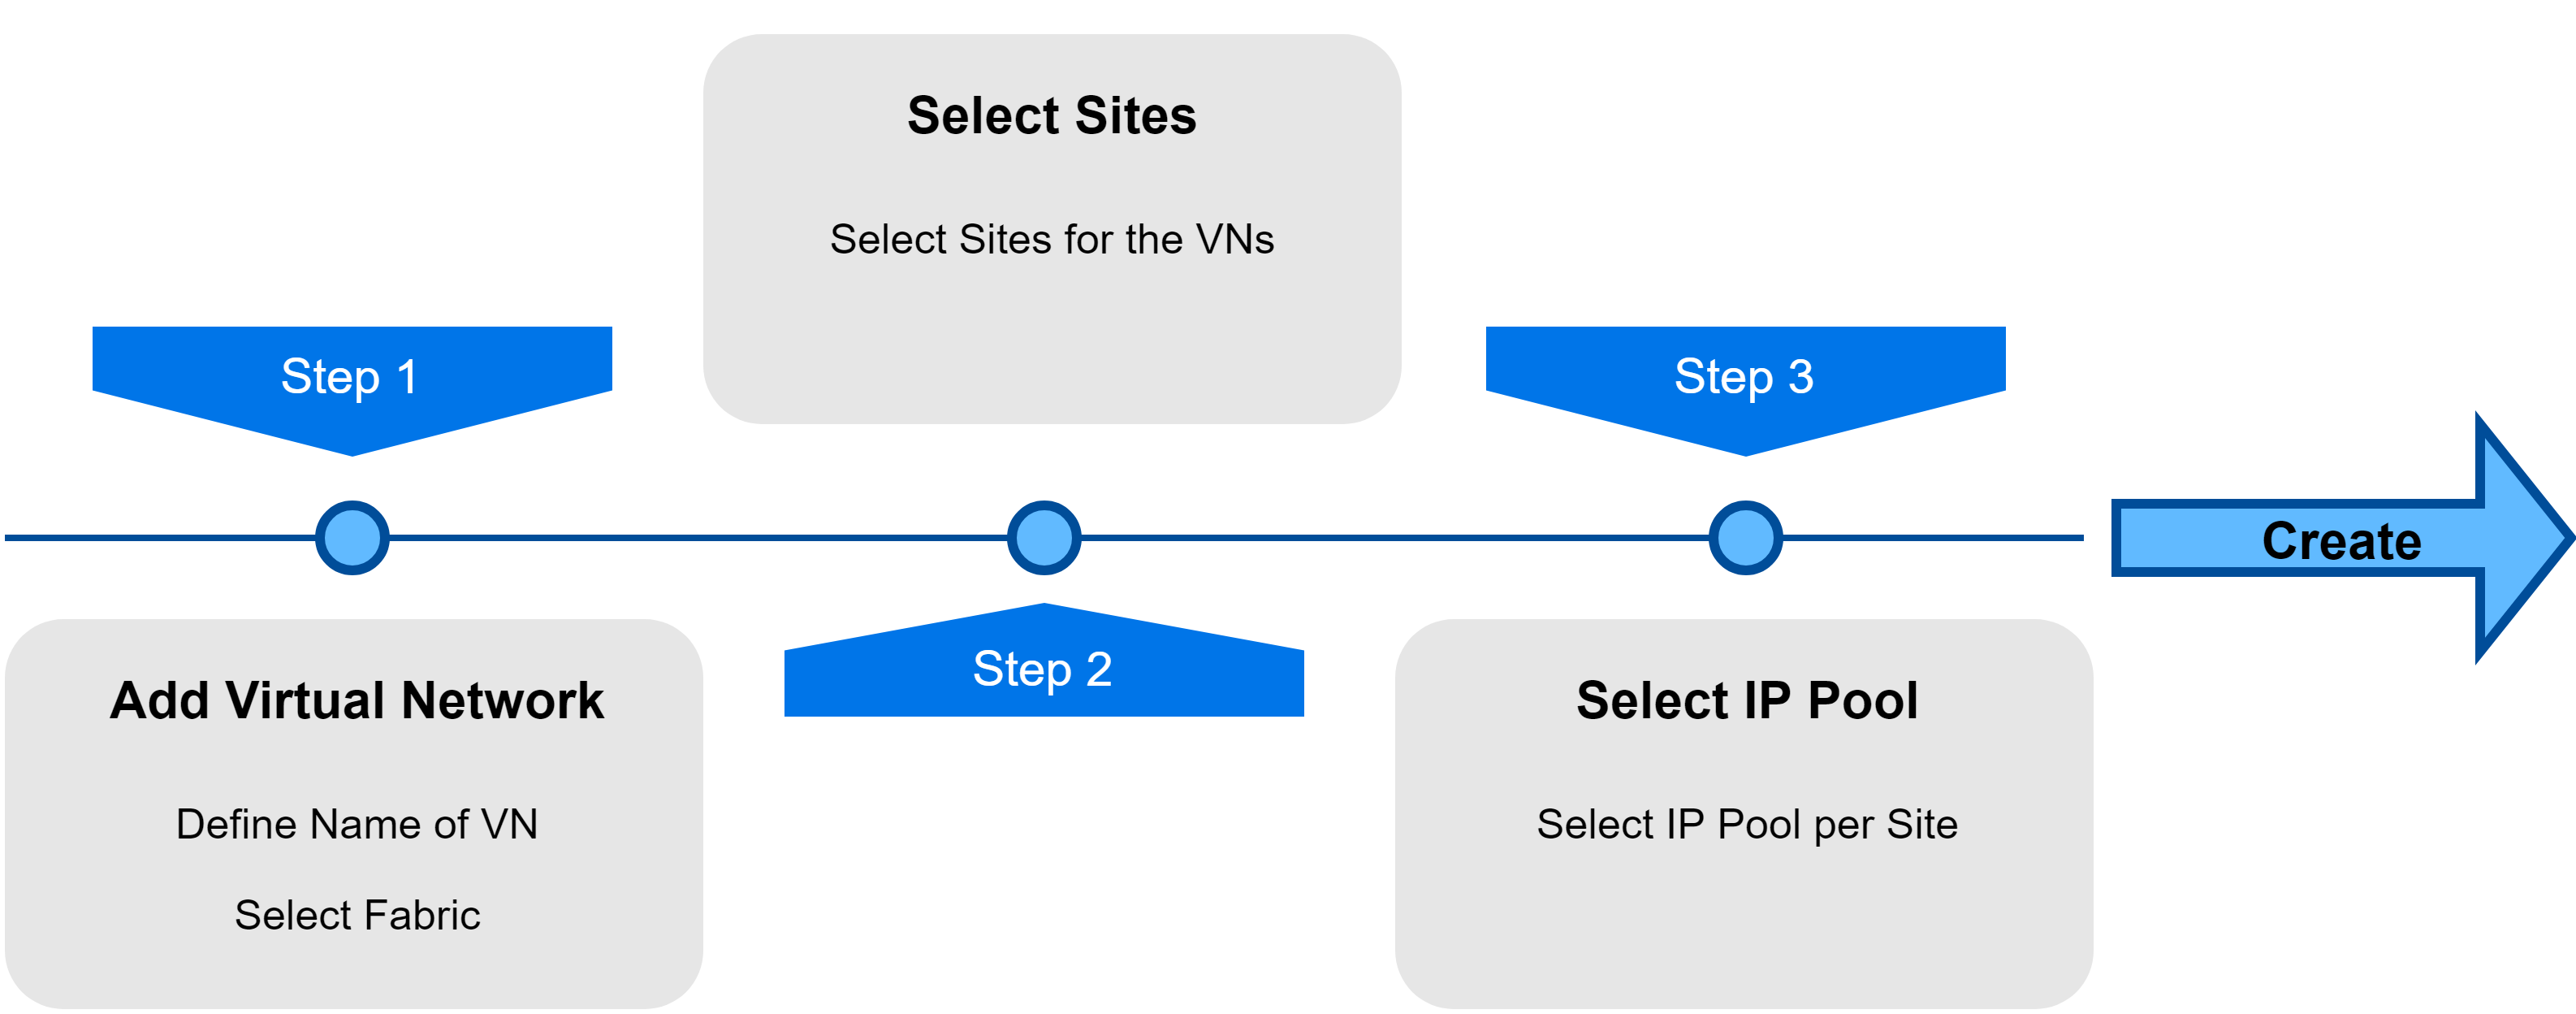
\includegraphics[width=0.8\linewidth]{img/Abstrahierung/addvirtualnetwork}
	\caption{Add Virtual Network}
	\label{fig:Add Virtual Network}
\end{figure}

Um den Wizard zu starten, kann im Orchestrationtool im Home \textit{Virtual Networks $\rightarrow$ Add Virtual Networks} ausgewählt werden. So startet der Wizard mit den in der Abbildung (siehe Abbildung \ref{fig:Add Virtual Network}: Add Virtual Network) aufgezeigten Schritten und man kann Schritt für Schritt die gewünschten Informationen angeben.

Der Wizard verwendet die APIs des DNA Centers, sowie der Netzwerkgeräte. Beim DNA Center mussten teilweise undokumentierte API Endpoints verwendet werden, da die nötigen Funktionen ansonsten nicht verfügbar sind. Dies birgt das Risiko, dass sich diese in Zukunft ändern und die Applikation angepasst werden muss.

\subsubsection{Virtual Machine Management}

Das Virtual Machine Management zeigt alle virtuallen Maschinen auf NFVIS an. Des Weiteren wird der aktuelle Status der VMs, sowie die Netzwerkinterfaces angezeigt. Zudem ist es möglich, eine VM über das Web Interface zu starten oder zu stoppen.

\begin{figure}[H]
	\centering
	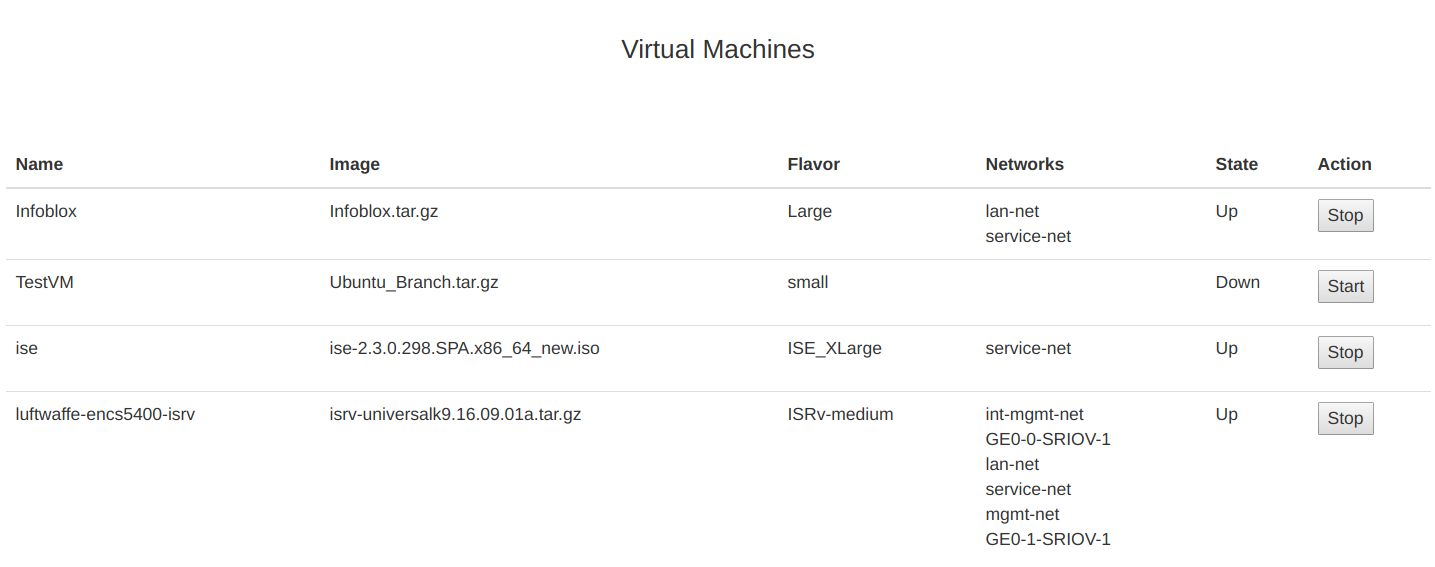
\includegraphics[width=0.8\linewidth]{img/Abstrahierung/vm-management.png}
	\caption{VM Management}
	\label{fig:VM Management}
\end{figure}

\subsubsection{Configuration History}

Dieser Use Case konnte nicht mehr vollständig umgesetzt werden. Derzeit kann nur die aktuelle Konfiguration angezeigt werden. Die Anzeige einer History ist noch nicht implementiert.

\begin{figure}[H]
	\centering
	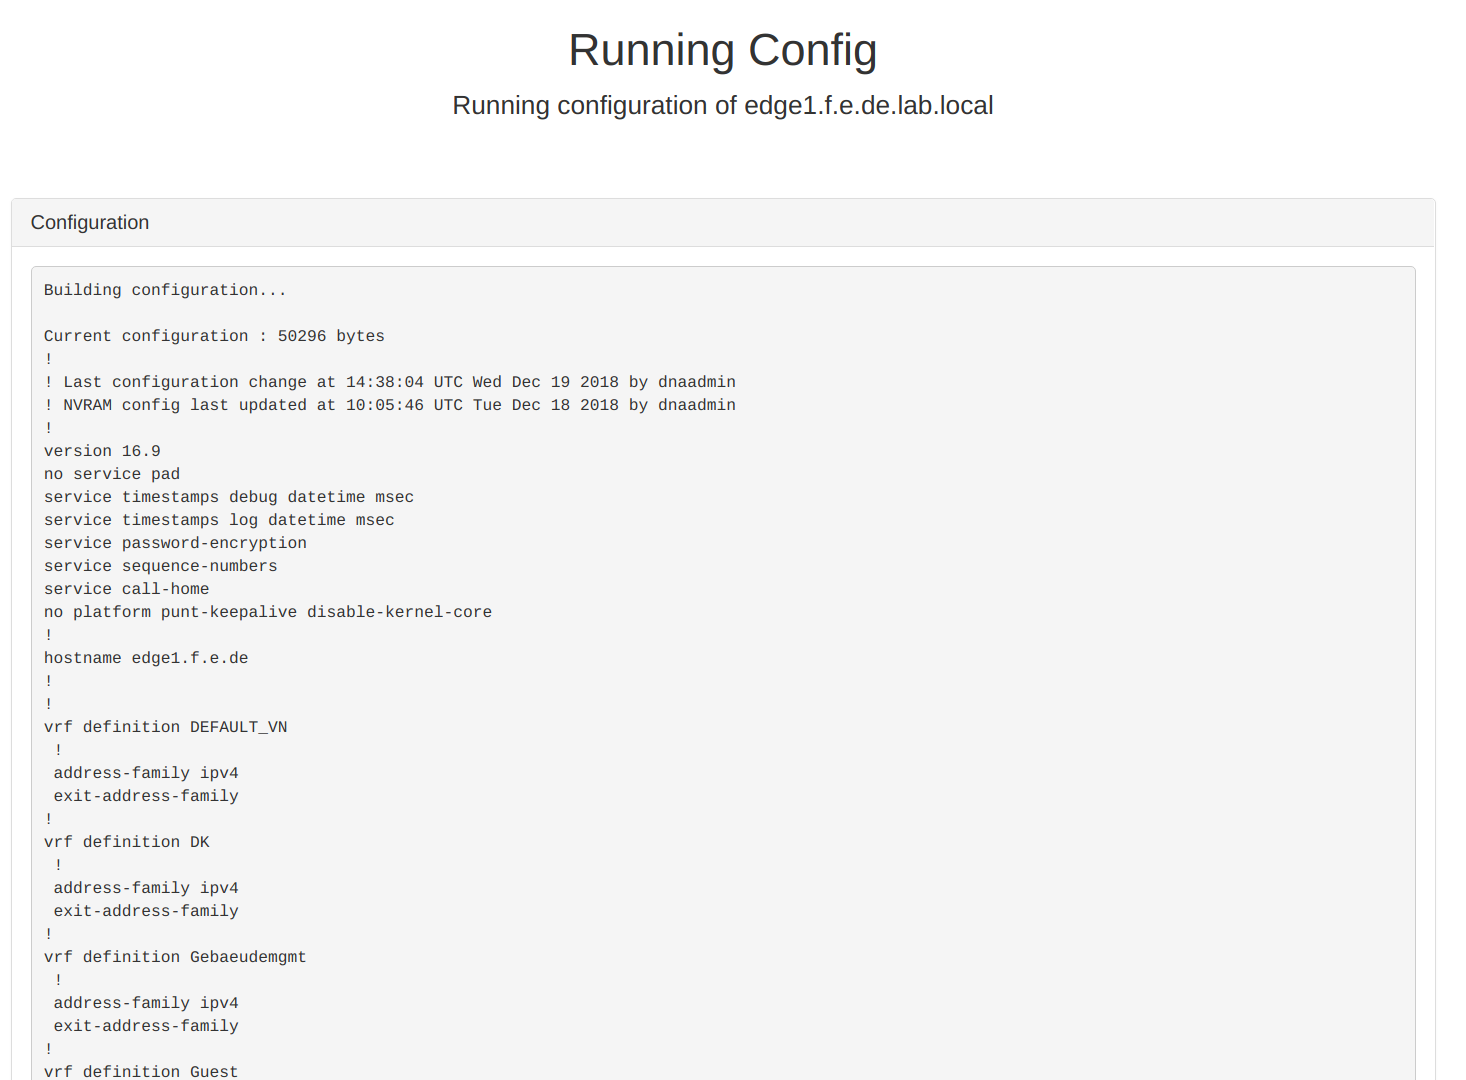
\includegraphics[width=0.8\linewidth]{img/Abstrahierung/running-config.png}
	\caption{Running Config}
	\label{fig:Running Config}
\end{figure}






